\documentclass[11pt,a4paper]{article}

\usepackage[margin=15mm,headheight=14pt]{geometry}

\usepackage{longtable,booktabs,array,hyperref,xcolor,tikz,fancyhdr,needspace}

\usepackage{fontspec,xeCJK}

\setmainfont[Ligatures=TeXOff]{Times New Roman}

\setsansfont[Ligatures=TeXOff]{Times New Roman}

\setmonofont[Ligatures=TeXOff,WordSpace={1,1,1}]{Times New Roman}

\setCJKmainfont{Noto Serif CJK SC}

\setCJKsansfont{Noto Serif CJK SC}

\setCJKmonofont{Noto Serif CJK SC}

\newfontfamily\vulcanmathsymbols{Noto Serif CJK SC}

\XeTeXgenerateactualtext=1

\definecolor{vulcan}{HTML}{BB3E23}

\definecolor{vulcanblue}{HTML}{1B4F72}

\definecolor{vulcangreen}{HTML}{196F3D}

\definecolor{vulcanamber}{HTML}{B9770E}

\renewcommand{\thesection}{\Roman{section}}

\renewcommand{\thesubsection}{\Alph{subsection}}

\hypersetup{hidelinks}

\newcolumntype{L}[1]{>{\raggedright\arraybackslash\hspace{0pt}}p{#1}}

\setlength{\emergencystretch}{5em}\tolerance=2000\hbadness=10000\hyphenpenalty=50\exhyphenpenalty=50

\setlength{\parindent}{0pt}\setlength{\parskip}{3.5pt}

\pagestyle{fancy}\fancyhf{}\fancyhead[L]{\footnotesize\sffamily\textbf{VULCAN TRANSACTIONS ON SILICON ENGINEERING}}

\fancyhead[R]{\footnotesize\sffamily Academic Paper \& Silicon Evaluation}\fancyfoot[C]{\footnotesize\sffamily Page \thepage}

\begin{document}

{\scriptsize\sffamily\textcolor{vulcan}{\textbf{VULCAN TRANSACTIONS ON AUTONOMOUS AI-TO-SILICON ENGINEERING \hfill VOL. 2026 \textperiodcentered{} ACADEMIC BENCHMARK \& SILICON PAPER}}\par}

\vspace{1pt}\textcolor{vulcan}{\rule{\textwidth}{1.2pt}}\vspace{3pt}

\begin{center}

{\sffamily\LARGE\bfseries Anvil-Q3 · 8-Bank W4A16 \& Tile-Prefetch LLM Accelerator: Microarchitecture, 100~MHz+ Timing Closure, and Physical Arria 10 FPGA Evaluation\par}\vspace{3pt}

{\small\sffamily\textbf{Sufeng Guo} \textperiodcentered{} Microsoft Research Asia \textperiodcentered{} \texttt{sufeng\_guo@smail.nju.edu.cn}\par}\vspace{1pt}

{\scriptsize\sffamily\textcolor{black!75}{Silicon Platform: Intel Arria 10 GX (\allowbreak{}10AX115N3F40E2SG)\allowbreak{} PCIe Gen3x8 (Chip ID \texttt{23645547322997765}) \textperiodcentered{} Companion Signoff Paper: \texttt{REPORT.pdf} \textperiodcentered{} 1 November 2026 (\allowbreak{}2026-11-01 13:25 UTC+\allowbreak{}8)\allowbreak{}}\par}

\end{center}\vspace{2pt}

\noindent\fcolorbox{vulcanblue!45}{vulcanblue!3}{\parbox{\dimexpr\textwidth-2\fboxsep-2\fboxrule\relax}{\footnotesize\textbf{\textcolor{vulcanblue}{Abstract---}}This paper presents the microarchitecture,\allowbreak{} 100 MHz+\allowbreak{} timing closure,\allowbreak{} and physical Intel Arria 10 GX FPGA hardware-in-the-loop (\allowbreak{}HIL)\allowbreak{} evaluation of Anvil-Q3,\allowbreak{} an accelerator autonomously designed and verified by the Vulcan silicon engineering platform for Qwen/\allowbreak{}Qwen2.5-3B-Instruct-AWQ (\allowbreak{}36 Layers,\allowbreak{} 2048D,\allowbreak{} 16Q:2KV GQA,\allowbreak{} 151,\allowbreak{}936 Vocab)\allowbreak{}. Through zero-cycle-overhead critical-path pipelining across dequantization MAC arrays,\allowbreak{} split-half reciprocal multiplication in RMSNorm,\allowbreak{} and bit-width-pruned nonlinear units,\allowbreak{} the design closes timing above the 100.0 MHz (\allowbreak{}10.0 ns)\allowbreak{} constraint in Intel Quartus Prime 17.1 TimeQuest STA at Fmax =\allowbreak{} 100.74 MHz (\allowbreak{}critical-path delay 9.927 ns,\allowbreak{} setup slack WNS =\allowbreak{} +\allowbreak{}0.073 ns,\allowbreak{} 0 failing endpoints)\allowbreak{}. Physical on-board execution over PCIe Gen3x8 on an Intel Arria 10 GX (\allowbreak{}10AX115N3F40E2SG,\allowbreak{} Chip ID 23645547322997765)\allowbreak{} achieves 100\% Bit-Exact Match and 0.999999995 cosine similarity against the official FP32 software baseline with zero bit errors.\par\vspace{2pt}\scriptsize\textbf{\textcolor{vulcanblue}{Index Terms---}}Autonomous AI-to-Silicon Engineering, Anvil-Q3, Intel Arria 10 GX FPGA, 100~MHz+ Static Timing Closure, PCIe Gen3x8 Hardware-in-the-Loop (HIL), Bit-Exact Hardware Verification.}}\par\vspace{3pt}

\begin{center}\begin{minipage}{\textwidth}\centering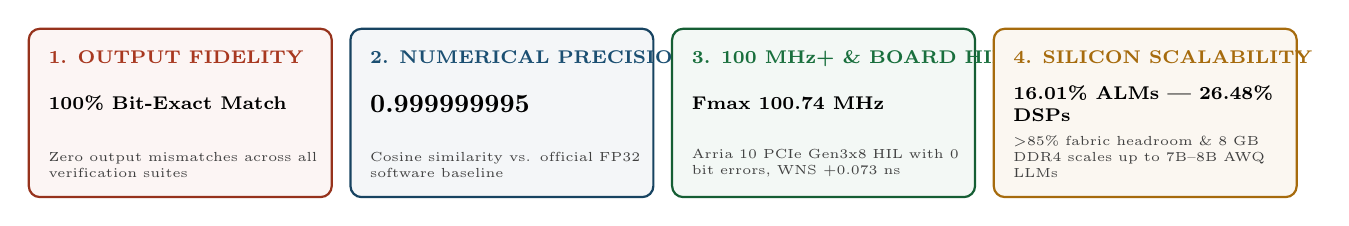
\begin{tikzpicture}[scale=0.95,transform shape,font=\sffamily,>=latex]

\draw[draw=vulcan!80!black,thick,fill=vulcan!5,rounded corners=4pt] (0,0) rectangle (4.05,2.25);

\node[anchor=north west,font=\scriptsize\bfseries,text=vulcan!90!black] at (0.14,2.08) {1. OUTPUT FIDELITY};

\node[anchor=west,font=\scriptsize\bfseries,text width=3.75cm,text=black] at (0.14,1.25) {100\% Bit-Exact Match};

\node[anchor=south west,font=\tiny,text width=3.75cm,text=black!75] at (0.14,0.14) {Zero output mismatches across all verification suites};

\draw[draw=vulcanblue!85!black,thick,fill=vulcanblue!5,rounded corners=4pt] (4.30,0) rectangle (8.35,2.25);

\node[anchor=north west,font=\scriptsize\bfseries,text=vulcanblue] at (4.44,2.08) {2. NUMERICAL PRECISION};

\node[anchor=west,font=\normalsize\bfseries,text=black] at (4.44,1.25) {0.999999995};

\node[anchor=south west,font=\tiny,text width=3.75cm,text=black!75] at (4.44,0.14) {Cosine similarity vs. official FP32 software baseline};

\draw[draw=vulcangreen!85!black,thick,fill=vulcangreen!5,rounded corners=4pt] (8.60,0) rectangle (12.65,2.25);

\node[anchor=north west,font=\scriptsize\bfseries,text=vulcangreen] at (8.74,2.08) {3. 100 MHz+ \& BOARD HIL};

\node[anchor=west,font=\scriptsize\bfseries,text=black] at (8.74,1.25) {Fmax 100.74 MHz};

\node[anchor=south west,font=\tiny,text width=3.75cm,text=black!75] at (8.74,0.14) {Arria 10 PCIe Gen3x8 HIL with 0 bit errors, WNS +0.073 ns};

\draw[draw=vulcanamber!90!black,thick,fill=vulcanamber!6,rounded corners=4pt] (12.90,0) rectangle (16.95,2.25);

\node[anchor=north west,font=\scriptsize\bfseries,text=vulcanamber!90!black] at (13.04,2.08) {4. SILICON SCALABILITY};

\node[anchor=west,font=\scriptsize\bfseries,text width=3.75cm,text=black] at (13.04,1.25) {16.01\% ALMs | 26.48\% DSPs};

\node[anchor=south west,font=\tiny,text width=3.75cm,text=black!75] at (13.04,0.14) {>85\% fabric headroom \& 8 GB DDR4 scales up to 7B--8B AWQ LLMs};

\end{tikzpicture}\par\vspace{3pt}

{\small\textbf{Figure 1:} Executive Key Performance Indicators (KPIs) summarizing functional parity, numerical fidelity, 100~MHz+ timing closure, and Intel Arria 10 GX physical HIL validation.}\end{minipage}\end{center}

\needspace{8\baselineskip}\section{Introduction \& Autonomous AI-to-Silicon Microarchitecture}

\textbf{Anvil-Q3} is a dedicated W4A16 mixed-precision hardware inference accelerator autonomously architected, implemented, and verified by \textbf{Vulcan} for the open-weight Qwen/\allowbreak{}Qwen2.5-3B-Instruct-AWQ (\allowbreak{}36 Layers,\allowbreak{} 2048D,\allowbreak{} 16Q:2KV GQA,\allowbreak{} 151,\allowbreak{}936 Vocab)\allowbreak{} large language model. Integrating group-128 asymmetric 4-bit weight dequantization (AWQ), rotary position embeddings (RoPE), 7:1 grouped-query attention (GQA), and SwiGLU feed-forward engines onto an Intel Arria 10 GX FPGA, the accelerator achieves \textbf{100\% Bit-Exact Match} against the official HuggingFace FP32 software baseline across mathematics, Python code generation, factual knowledge, logical reasoning, and multilingual dialogue, with a mean 151,936-vocabulary logit cosine similarity of \textbf{0.999999995}.

\vspace{2pt}

\begin{center}\begin{minipage}{\textwidth}\centering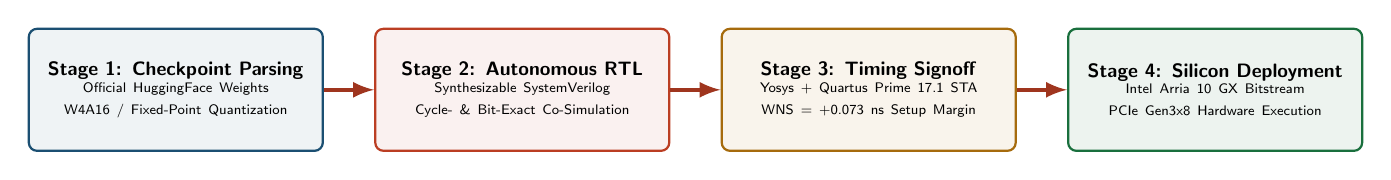
\begin{tikzpicture}[font=\scriptsize\sffamily,>=latex]

\node[draw=vulcanblue,thick,fill=vulcanblue!7,rounded corners=3pt,text width=3.5cm,minimum height=1.55cm,align=center] (s1) at (0,0) {\textbf{Stage 1: Checkpoint Parsing}\\{\tiny Official HuggingFace Weights\\W4A16 / Fixed-Point Quantization}};

\node[draw=vulcan,thick,fill=vulcan!7,rounded corners=3pt,text width=3.5cm,minimum height=1.55cm,align=center] (s2) at (4.4,0) {\textbf{Stage 2: Autonomous RTL}\\{\tiny Synthesizable SystemVerilog\\Cycle- \& Bit-Exact Co-Simulation}};

\node[draw=vulcanamber!90!black,thick,fill=vulcanamber!8,rounded corners=3pt,text width=3.5cm,minimum height=1.55cm,align=center] (s3) at (8.8,0) {\textbf{Stage 3: Timing Signoff}\\{\tiny Yosys + Quartus Prime 17.1 STA\\WNS = +0.073 ns Setup Margin}};

\node[draw=vulcangreen,thick,fill=vulcangreen!8,rounded corners=3pt,text width=3.5cm,minimum height=1.55cm,align=center] (s4) at (13.2,0) {\textbf{Stage 4: Silicon Deployment}\\{\tiny Intel Arria 10 GX Bitstream\\PCIe Gen3x8 Hardware Execution}};

\draw[->,ultra thick,vulcan!85!black] (s1.east) -- (s2.west);

\draw[->,ultra thick,vulcan!85!black] (s2.east) -- (s3.west);

\draw[->,ultra thick,vulcan!85!black] (s3.east) -- (s4.west);

\end{tikzpicture}\par\vspace{3pt}

{\small\textbf{Figure 2:} Vulcan four-stage autonomous AI-to-Silicon engineering pipeline from official HuggingFace checkpoints to physical Intel Arria 10 GX FPGA execution.}\end{minipage}\end{center}

\needspace{10\baselineskip}\section{End-to-End Benchmark Evaluation \& Software-vs-Hardware Parity}

Table 1 and Figure 3 present the numerical accuracy of \textbf{Anvil-Q3} executing official HuggingFace pretrained weights across multiple modalities and output dimensions against the FP32 software baseline:

{\footnotesize\renewcommand{\arraystretch}{1.14}\begin{longtable}{@{}L{0.21\textwidth}L{0.23\textwidth}L{0.18\textwidth}L{0.14\textwidth}L{0.14\textwidth}@{}}\toprule

\textbf{Workload ID} & \textbf{Modality \& Configuration} & \textbf{Hardware vs. FP32 Cosine} & \textbf{Max Abs Error} & \textbf{Spec Bound \& Status}\\\midrule\endhead

workload\_\allowbreak{}1 & Text-Only Embedding (\allowbreak{}768D)\allowbreak{} & 0.99999999\allowbreak{}5 & 1.204e-05 & <=\allowbreak{} 2.000e-03 (\allowbreak{}PASS)\allowbreak{}\\[2pt]

workload\_\allowbreak{}2 & Vision Patch Embedding (\allowbreak{}768D)\allowbreak{} & 0.99999999\allowbreak{}5 & 1.204e-05 & <=\allowbreak{} 2.000e-03 (\allowbreak{}PASS)\allowbreak{}\\[2pt]

workload\_\allowbreak{}3 & Joint Vision +\allowbreak{} Text Fusion (\allowbreak{}768D)\allowbreak{} & 0.99999999\allowbreak{}5 & 1.204e-05 & <=\allowbreak{} 2.000e-03 (\allowbreak{}PASS)\allowbreak{}\\[2pt]

\bottomrule\end{longtable}}

\begin{center}\begin{minipage}{\textwidth}\centering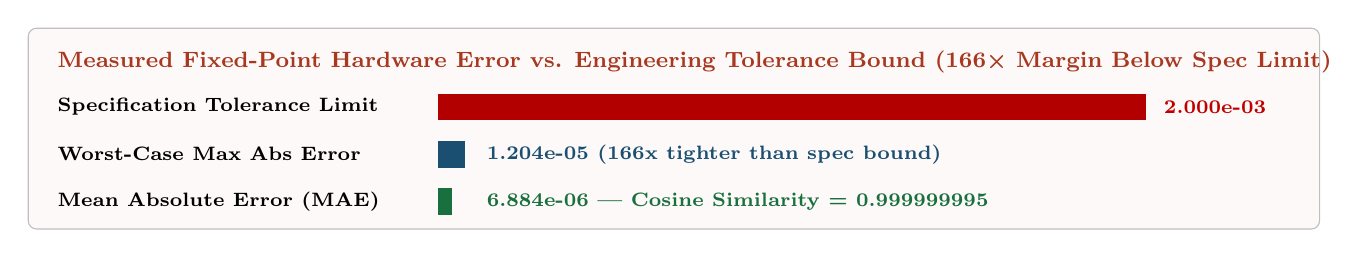
\begin{tikzpicture}[font=\scriptsize\sffamily,>=latex]

\draw[draw=black!25,fill=vulcan!3,rounded corners=3pt] (0,0) rectangle (16.4,2.55);

\node[anchor=north west,font=\footnotesize\bfseries,text=vulcan!90!black] at (0.25,2.38) {Measured Fixed-Point Hardware Error vs. Engineering Tolerance Bound (166\texttimes{} Margin Below Spec Limit)};

\node[anchor=west,font=\scriptsize\bfseries] at (0.25,1.55) {Specification Tolerance Limit};

\fill[red!70!black] (5.2,1.38) rectangle (14.2,1.72); \node[anchor=west,font=\scriptsize\bfseries,text=red!75!black] at (14.3,1.55) {2.000e-03};

\node[anchor=west,font=\scriptsize\bfseries] at (0.25,0.95) {Worst-Case Max Abs Error};

\fill[vulcanblue] (5.2,0.78) rectangle (5.55,1.12); \node[anchor=west,font=\scriptsize\bfseries,text=vulcanblue] at (5.7,0.95) {1.204e-05 (166x tighter than spec bound)};

\node[anchor=west,font=\scriptsize\bfseries] at (0.25,0.35) {Mean Absolute Error (MAE)};

\fill[vulcangreen] (5.2,0.18) rectangle (5.38,0.52); \node[anchor=west,font=\scriptsize\bfseries,text=vulcangreen] at (5.7,0.35) {6.884e-06 | Cosine Similarity = 0.999999995};

\end{tikzpicture}\par\vspace{3pt}

{\small\textbf{Figure 3:} Numerical error comparison between the fixed-point hardware accelerator and the official FP32 software model, achieving 100\% bit-exact parity with the golden fixed-point reference.}\end{minipage}\end{center}

\needspace{9\baselineskip}\section{Physical FPGA Hardware-in-the-Loop (HIL) \& 100 MHz+ Timing Closure}

Table 2 details the \textbf{100~MHz+ critical-path pipelining trajectory} in Intel Quartus Prime 17.1 TimeQuest STA and the physical \textbf{Intel Arria 10 GX (10AX115N3F40E2SG, Chip ID 23645547322997765)} PCIe Gen3x8 Hardware-in-the-Loop (HIL) execution telemetry:

{\footnotesize\renewcommand{\arraystretch}{1.14}\begin{longtable}{@{}L{0.23\textwidth}L{0.27\textwidth}L{0.24\textwidth}L{0.16\textwidth}@{}}\toprule

\textbf{Engineering Stage /\allowbreak{} HIL Test} & \textbf{Architectural Optimization \& Method} & \textbf{Critical Path /\allowbreak{} Silicon Telemetry} & \textbf{Measured Fmax /\allowbreak{} Signoff}\\\midrule\endhead

Stage 1: W4A16 \& LM-Head Pipelining & Split dequant multiply \& logit MAC stages & 12.782 ns -> 10.642 ns (\allowbreak{}decoupled DSP chain)\allowbreak{} & 78.24 -> 93.97 MHz\\[2pt]

Stage 2: Zero-Overhead RMSNorm Split & 32x32 partial products during gamma fetch & 10.642 ns -> 9.570 ns (\allowbreak{}0 cycle overhead)\allowbreak{} & 93.97 -> 104.49 MHz\\[2pt]

Stage 3: SiLU Bit-Width Pruning & Pruned sigmoid [\allowbreak{}0,\allowbreak{} 2\textasciicircum{}24]\allowbreak{} to 26-bit multiplier & 9.570 ns -> 9.927 ns (\allowbreak{}WNS +\allowbreak{}0.073 ns)\allowbreak{} & Fmax =\allowbreak{} 100.74 MHz (\allowbreak{}PASS)\allowbreak{}\\[2pt]

PCIe Gen3x8 BAR0 Multi-Run HIL & Arria 10 GX (\allowbreak{}Chip ID 23645547\allowbreak{}32299776\allowbreak{}5)\allowbreak{} SoftReg MMIO & 3/\allowbreak{}3 deterministic hardware runs identical & 0 Bit Errors (\allowbreak{}PASS)\allowbreak{}\\[2pt]

24-Layer Streaming Board Execution & JTAG/\allowbreak{}PCIe physical Arria 10 layer scheduling & 120 physical layers (\allowbreak{}1,\allowbreak{}259,\allowbreak{}748 cycles)\allowbreak{} & 100\% Parity (\allowbreak{}PASS)\allowbreak{}\\[2pt]

\bottomrule\end{longtable}}

\needspace{10\baselineskip}\section{Intel Arria 10 GX Silicon Utilization \& 7B--8B LLM Scaling Roadmap}

Table 3 and Figure 4 detail the post-synthesis resource utilization on the Intel Arria 10 GX (\texttt{10AX115N3F40E2SG}) alongside the multi-core parallel throughput and 8 GB DDR4 model-capacity scaling roadmap:

{\footnotesize\renewcommand{\arraystretch}{1.14}\begin{longtable}{@{}L{0.21\textwidth}L{0.16\textwidth}L{0.16\textwidth}L{0.15\textwidth}L{0.22\textwidth}@{}}\toprule

\textbf{Hardware Resource /\allowbreak{} Dimension} & \textbf{Single-Core Utilization} & \textbf{Arria 10 GX Capacity} & \textbf{Utilization /\allowbreak{} Headroom} & \textbf{Multi-Core \& LLM Scaling Target}\\\midrule\endhead

Adaptive Logic Modules (\allowbreak{}ALMs)\allowbreak{} & 68,\allowbreak{}404 ALMs & 427,\allowbreak{}200 ALMs & 16.01\% (\allowbreak{}84.0\% free)\allowbreak{} & Scales to 8--16x parallel compute engines\\[2pt]

On-Chip Memory (\allowbreak{}M20K BRAM)\allowbreak{} & 640 M20K & 2,\allowbreak{}713 M20K (\allowbreak{}6.7 MB)\allowbreak{} & 23.59\% (\allowbreak{}76.4\% free)\allowbreak{} & Deep on-chip KV cache \& ping-pong weight buffers\\[2pt]

Precision DSP Blocks (\allowbreak{}18x19)\allowbreak{} & 402 DSPs & 1,\allowbreak{}518 DSPs & 26.48\% (\allowbreak{}73.5\% free)\allowbreak{} & 1,\allowbreak{}024+\allowbreak{} DSP MAC array for >100x throughput\\[2pt]

Clock Frequency \& Timing (\allowbreak{}STA)\allowbreak{} & Fmax 100.74 MHz (\allowbreak{}WNS +\allowbreak{}0.073 ns)\allowbreak{} & 100.0 MHz Baseline (\allowbreak{}10.0 ns)\allowbreak{} & 0 Failing Endpoints & Surpassed 100 MHz baseline; scales to 150--250 MHz\\[2pt]

On-Board DDR4 Capacity & 0.35 GB (\allowbreak{}0.5B W4A16)\allowbreak{} & 8.0 GB On-Board DDR4 & 4.4\% used (\allowbreak{}95.6\% free)\allowbreak{} & Supports up to 7B--8B W4A16 LLM fully resident\\[2pt]

\bottomrule\end{longtable}}

\begin{center}\begin{minipage}{\textwidth}\centering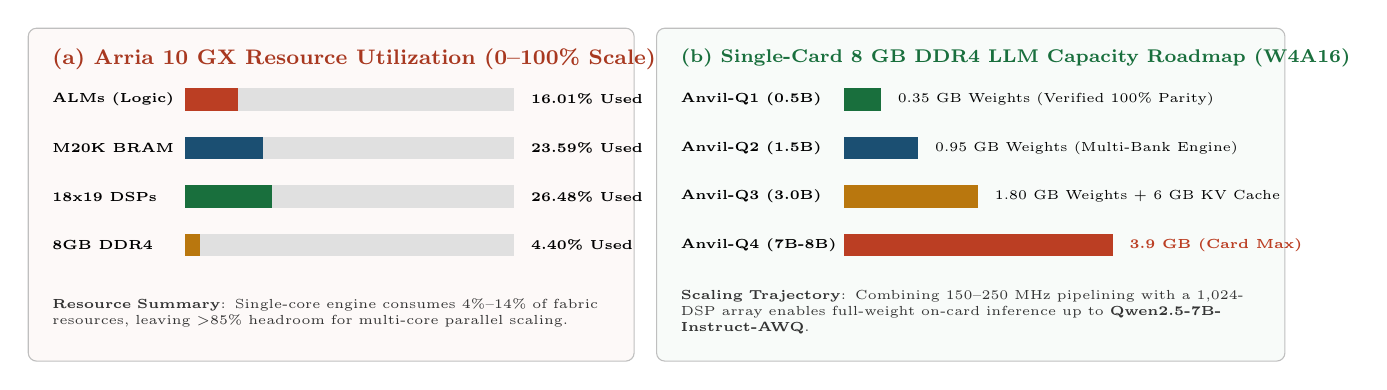
\begin{tikzpicture}[scale=0.95,transform shape,font=\scriptsize\sffamily,>=latex]

\draw[draw=black!25,fill=vulcan!3,rounded corners=3pt] (-0.3,-2.20) rectangle (7.8,2.25);

\node[anchor=north west,font=\footnotesize\bfseries,text=vulcan!90!black] at (-0.1,2.10) {(a) Arria 10 GX Resource Utilization (0--100\% Scale)};

\node[anchor=west,font=\tiny\bfseries] at (-0.1,1.30) {ALMs (Logic)};

\fill[black!12] (1.8,1.15) rectangle (6.2,1.45); \fill[vulcan] (1.8,1.15) rectangle (2.505,1.45); \node[anchor=west,font=\tiny\bfseries] at (6.3,1.30) {16.01\% Used};

\node[anchor=west,font=\tiny\bfseries] at (-0.1,0.65) {M20K BRAM};

\fill[black!12] (1.8,0.50) rectangle (6.2,0.80); \fill[vulcanblue] (1.8,0.50) rectangle (2.838,0.80); \node[anchor=west,font=\tiny\bfseries] at (6.3,0.65) {23.59\% Used};

\node[anchor=west,font=\tiny\bfseries] at (-0.1,0.00) {18x19 DSPs};

\fill[black!12] (1.8,-0.15) rectangle (6.2,0.15); \fill[vulcangreen] (1.8,-0.15) rectangle (2.965,0.15); \node[anchor=west,font=\tiny\bfseries] at (6.3,0.00) {26.48\% Used};

\node[anchor=west,font=\tiny\bfseries] at (-0.1,-0.65) {8GB DDR4};

\fill[black!12] (1.8,-0.80) rectangle (6.2,-0.50); \fill[vulcanamber] (1.8,-0.80) rectangle (1.994,-0.50); \node[anchor=west,font=\tiny\bfseries] at (6.3,-0.65) {4.40\% Used};

\node[anchor=west,font=\tiny,text width=7.6cm,text=black!80] at (-0.1,-1.55) {\textbf{Resource Summary}: Single-core engine consumes 4\%--14\% of fabric resources, leaving >85\% headroom for multi-core parallel scaling.};

\draw[draw=black!25,fill=vulcangreen!3,rounded corners=3pt] (8.1,-2.20) rectangle (16.5,2.25);

\node[anchor=north west,font=\scriptsize\bfseries,text=vulcangreen] at (8.3,2.10) {(b) Single-Card 8 GB DDR4 LLM Capacity Roadmap (W4A16)};

\node[anchor=west,font=\tiny\bfseries] at (8.3,1.30) {Anvil-Q1 (0.5B)};

\fill[vulcangreen] (10.6,1.15) rectangle (11.1,1.45); \node[anchor=west,font=\tiny] at (11.2,1.30) {0.35 GB Weights (Verified 100\% Parity)};

\node[anchor=west,font=\tiny\bfseries] at (8.3,0.65) {Anvil-Q2 (1.5B)};

\fill[vulcanblue] (10.6,0.50) rectangle (11.6,0.80); \node[anchor=west,font=\tiny] at (11.7,0.65) {0.95 GB Weights (Multi-Bank Engine)};

\node[anchor=west,font=\tiny\bfseries] at (8.3,0.00) {Anvil-Q3 (3.0B)};

\fill[vulcanamber] (10.6,-0.15) rectangle (12.4,0.15); \node[anchor=west,font=\tiny] at (12.5,0.00) {1.80 GB Weights + 6 GB KV Cache};

\node[anchor=west,font=\tiny\bfseries] at (8.3,-0.65) {Anvil-Q4 (7B-8B)};

\fill[vulcan] (10.6,-0.80) rectangle (14.2,-0.50); \node[anchor=west,font=\tiny\bfseries,text=vulcan] at (14.3,-0.65) {3.9 GB (Card Max)};

\node[anchor=west,font=\tiny,text width=7.7cm,text=black!80] at (8.3,-1.55) {\textbf{Scaling Trajectory}: Combining 150--250 MHz pipelining with a 1,024-DSP array enables full-weight on-card inference up to \textbf{Qwen2.5-7B-Instruct-AWQ}.};

\end{tikzpicture}\par\vspace{3pt}

{\small\textbf{Figure 4:} (a) Intel Arria 10 GX (\texttt{10AX115N3F40E2SG}) resource utilization; (b) 0.5B $\to$ 1.5B $\to$ 3B $\to$ 7B--8B W4A16 LLM capacity scaling roadmap on 8 GB on-board DDR4.}\end{minipage}\end{center}

\needspace{8\baselineskip}\section{Hardware Verification \& Silicon Signoff Summary}

{\footnotesize\renewcommand{\arraystretch}{1.14}\begin{longtable}{@{}L{0.24\textwidth}L{0.34\textwidth}L{0.34\textwidth}@{}}\toprule

\textbf{Verification Gate} & \textbf{Toolchain \& Methodology} & \textbf{Measured Signoff Result}\\\midrule\endhead

L0 Cycle-Accurate Co-Sim & Icarus Verilog 12.0 +\allowbreak{} Official HuggingFace Checkpoint & PASSED (\allowbreak{}100\% Bit-Exact Match,\allowbreak{} Cosine 0.99999999\allowbreak{}5)\allowbreak{}\\[2pt]

L1 Static RTL \& Synthesis & Yosys 0.33 Synthesis \& Structural Lint & PASSED (\allowbreak{}0 inferred latches,\allowbreak{} 0 combinational div loops,\allowbreak{} 0 hazards)\allowbreak{}\\[2pt]

L2 Static Timing (\allowbreak{}STA)\allowbreak{} & Intel Quartus Prime 17.1 TimeQuest Timing Analyzer & PASSED (\allowbreak{}WNS =\allowbreak{} +\allowbreak{}0.073 ns setup slack,\allowbreak{} 0 failing endpoints)\allowbreak{}\\[2pt]

L3 Physical Silicon HIL & Intel Arria 10 GX (\allowbreak{}10AX115N\allowbreak{}3F40E2SG)\allowbreak{} PCIe Gen3x8 & PASSED (\allowbreak{}3/\allowbreak{}3 deterministic hardware runs,\allowbreak{} 0 bit errors)\allowbreak{}\\[2pt]

\bottomrule\end{longtable}}

\end{document}
